\begin{figure*}
    \centering
    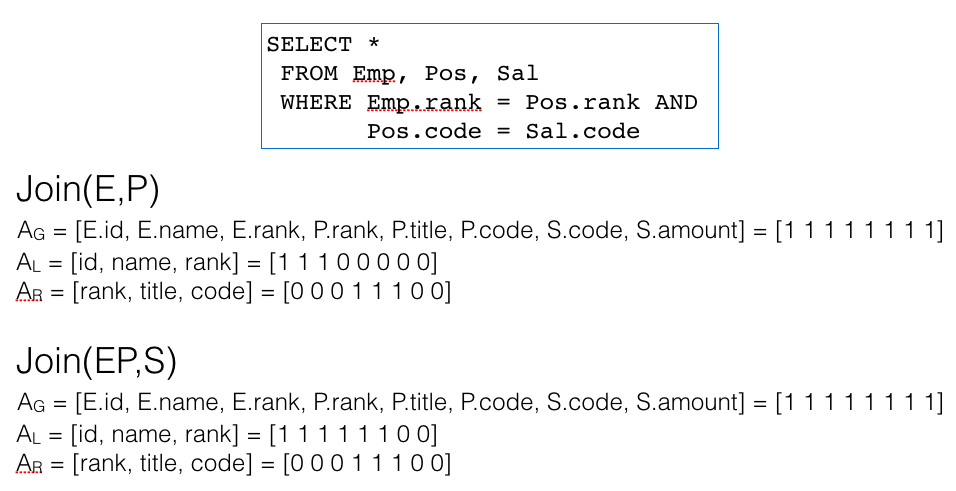
\includegraphics[width=0.7\textwidth]{figs/featurization.png}
    \caption{We use 1-hot encoding to capture which attributes participate in a join. This allows us to featurize both the query graph and the contraction. This figure shows the featurization for two different joins for the example query. \zongheng{I can try to plot this in LaTex.} \label{feat}}
\end{figure*}

\begin{figure}
    \centering
    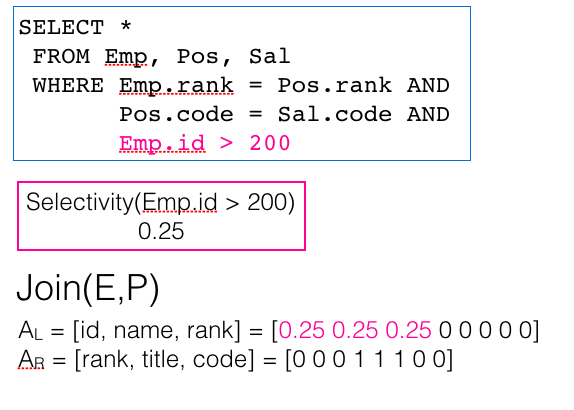
\includegraphics[width=0.8\columnwidth]{figs/selectivity.png}
    \caption{To featurize single table selections, we scale the features by selectivity estimates given to use from a cost-estimator. \zongheng{I can try to plot this in LaTex.} \label{feat:sel}}
\end{figure}

\begin{figure}
    \centering
    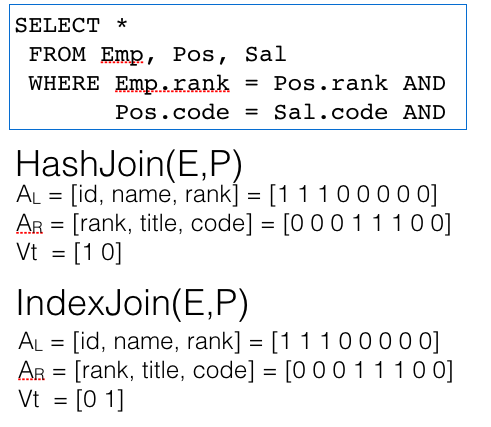
\includegraphics[width=0.8\columnwidth]{figs/type.png}
    \caption{To featurize join types, we add another feature vector to indicate the type of join used. For example, in a system that choses between index joins and hash joins, the example queries features would include the above vectors. \zongheng{I can try to plot this in LaTex.} \label{feat:type}}
\end{figure}

\section{Learning to Optimize}
To be able to learn the Q function, we need two pieces: featurized representation for the arguments ($G$ and $c$) and a way of collecting training data.

\subsection{Featurizing the Join Decision}
We need to featurize the query graph $G$ and a particular contraction $c$, which is a tuple of two vertices from the graph. 

\vspace{0.5em} \noindent \textbf{Participating Relations: } The first step is to construct a set of features to represent which relations are participating the in the query and in the particular contraction. Let $A$ be the set of all attributes in the database (e.g., $ \{Emp.id, Pos.rank,...,Sal.code,Sal.amount\}$). Each relation $r$ (including intermediate relations that are the result of join) has a set of \emph{visible attributes}; those attributes present in the output $A_r \subseteq A$. So every query graph $G$ can be represented by its visible attributes $A_G$. Each contraction is a tuple of two relations $(l,r)$ and we can get the visible attributes $A_l$ and $A_r$ for each. Each of these subsets $A_G, A_l, A_r$ can be represented with a binary 1-hot encoding representing which subset of the attributes are present. We call the concatenation of these vectors $V_{rel}$ and it has dimensionality of $3\cdot|A|$. Figure \ref{feat} illustrates the featurization on the example query in the background section. 

To handle single relation selections in the query, we have to tweak the feature representation. This is because upstream selections and projections will change the cost properties of downstream joins. As in the classical optimizers, we eagerly apply selections and projections to each relation. 
Here, we leverage the table statistics present in most RDBMS. For each relation in the query graph, we can estimate a reduction factor $\delta_{r}$, which is an estimate of the fraction of tuples present after applying the selection to relation $r$. 
In the featurization described in the previous section, we have a set of binary features $V_{rel}$ that describe the participating attributes.
We multiply the reduction factors $\delta_r$ for each table with the features corresponding to attributes derived from that relation.
Figure \ref{feat:sel} illustrates the effect of adding a single table predicate to the example query. 

\vspace{0.5em} \noindent \textbf{Physical Operator: } The next piece is to featurize the join condition and the choice of physical operator. Handling the physical operator is easy; we simply add another feature that indicates from a dictionary what type of a join was used. We call this vector $V_{type}$. Figure \ref{feat:type} illustrates the effect of modeling physical operators. 

\vspace{0.5em} \noindent \textbf{Extensibility: } In the paper, we present the most basic form of featurization. Any property that we want the model to capture and believe is relevant to predicting the cost of a join can be added to the feature representation.  For example, we can add an addition set of binary features $V_{ind}$ that indicate which attributes have indexes built on them. Handling, sort-orders are similar and we have to add features describing which attributes need to be finally sorted in the query. We can similarly add features that describe the available memory if we believe that is an important resource to manage in determining the final best plan.

\subsection{Generating the Training Data}
The Q-function is represented as a multi-layer perceptron (MLP) neural network.
It takes as input two feature vectors $V_{rel}$ and $V_{type}$. Experimentally, we found that a two-layer MLP gave the best performance relative to the training time. We implmented the training algorithm in \textsf{DL4J} a java framework for model training with a standard DQN algorithm. 

Now, we describe what kind of training data is necessary to learn a Q-function. In supervised regression, we collect data of the form \texttt{(feature, values)}. The learned function maps from feature to values. One can think of this as a \emph{stateless} prediction, where the underlying prediction problem does not depend on some underlying process state. On the other hand, in the Q-Learning setting, there is state. So we have to collect training data of the form \texttt{(state, decision, new state, cost)}. Therefore, in our setting a training dataset consists of tuples of the following format:
\begin{lstlisting}
List<Graph, Join, New Graph, Cost> dataset;
\end{lstlisting}
or \texttt{(G, c, G', J)} for short. This defines a stochastic gradient descent iteration until convergence:
\[
\theta^{(i+1)} \leftarrow \theta^{(i)} - \alpha \cdot [ (J + \min_{c'} Q_\theta(G',c')) - Q_\theta(G,c) ] \cdot \nabla_\theta Q_\theta(G,c) 
\]
Q-Learning is known as an off-policy RL method. This means that its training is independent of the data collection process and can be suboptimal--as long as the data collection process sufficiently covers relevant scenarios. 

Such data can be collected from querying an optimizer's native cost model. In fact, the data is \emph{automatically generated} as a consequence of running classical planning algorithms. For example, if we run a classical dynamic programming algorithm to optimize a k-way join, we not only get $\texttt{(G, c, G', J)}$ samples along the final join path but every single subplan enumerated along the way! Any such optimizer can be used: bushy trees, zig-zag trees, left-deep, or right-deep. Randomized algorithms such as QuickPick~\cite{waas2000join} can also be used to generate training data. 

In our experiments, we bootstrap planning with a bushy dynamic programming optimizer until the number of relations in the join exceeds 9 relations.  Then, the data generation algorithm switches to a greedy scheme for efficiency for the first $K-9$ joins.
Ironically, the data collected from such an optimizer might be ``too good''.
The learned Q-function is only an approximation of the optimizer's true cost-to-go table, and thus, during execution branches of the tree not expanded by the optimizer in training can be an issue.
If the training data only consisted of optimal plans, then the learned Q-function may not accurately score poor plans. Likewise, if the training purely sampled random plans--it may not see very many instances of good plans.
During data collection noise can be injected into the planner to force it to enumerate diverse set of subplans.
The way that we implement this is to have a probabilistic parameter $\epsilon$ that randomizes the replacement policy in the memoization table.
As the algorithm enumerates more subplans, if a particular relation set exists in the table it replaces the access path if the enumerated plan has a lower cost than one in the table and with $\textsf{rand()} > \epsilon$.

\subsection{Execution after Training}
After training, we will have a parametrized estimate of the Q-function, $Q_\theta(f_G,f_c)$. For execution, we simply go back to the standard algorithm as in the greedy method but instead of using the local costs, we use the learned Q-function: (1) start with the query graph, (2) featurize each contraction (2) find the contraction with the lowest \textbf{estimated Q-value}, (3) update the query graph and repeat.
This algorithm has the time-complexity of greedy enumeration except in greedy the cost model is evaluated at each iteration, and in our method, a neural network is evaluated. Neural network evaluation can heavily leverage vectorization. In each iteration of the algorithm, we generate features corresponding to each contraction. Rather than evaluating the neural network on each, we can evaluate them on the entire batch. Modern architectures are designed to efficiently do such numerical computation and execution can be even faster leveraging specialized hardware like Graphics Processing Units and Tensor Processing Units.

\subsection{Feedback From Execution}
A learned Q-function also allows us to leverage feedback from real query executions.
Readers might be familiar with the concept of fine-tuning in the neural network literature~\cite{yosinski2014transferable}, where a network is trained on one dataset and transferred to another with minimal retraining.
We can apply a very similar principle to accounting for feedback.

The Q-function relates subplans to future projected costs.
As with any cost model, the cumulative cost is a proxy for runtime.
We can define a new cost function where the immediate cost of all joins are 0 but the cost of the final plan is its runtime.
We can generate a fine-tuning dataset $\{x_i\}_i^N$ with:
\[
x_i = \begin{cases}
\texttt{(G, c, G', 0)} \text{ if not final},\\
\texttt{(G, c, G',~runtime)} \text{ else}\\
\end{cases}
\]

To train this model, we can pre-train the network on a large amount of samples from the optimizer's cost model. 
These samples are inexpensive compared to execution.
We train the model on these samples to convergence.
Then, we freeze the weights of the first two layers, and re-initialize the last layer (also called the output layer).
We retrain this layer with a small amount of execution data collected.

One can think about the fine-tuning process as first using the cost model to learn relevant features about the structure suplans (i.e., which ones are generally beneficial). After this is learned, those features are fed into a predictor to project the effect of that decision on final runtime. 